
\chapter{Sampling-based Inference}

Our focus in this chapter is on solving inference based problems by sampling strategies. This is needed because in the context of Bayesian Networks we are only able to perform inference if our network satisfies certain structural properties; in particular it has to be a tree or a poli-tree. 

Even in a simple exampl like 

\begin{center}
    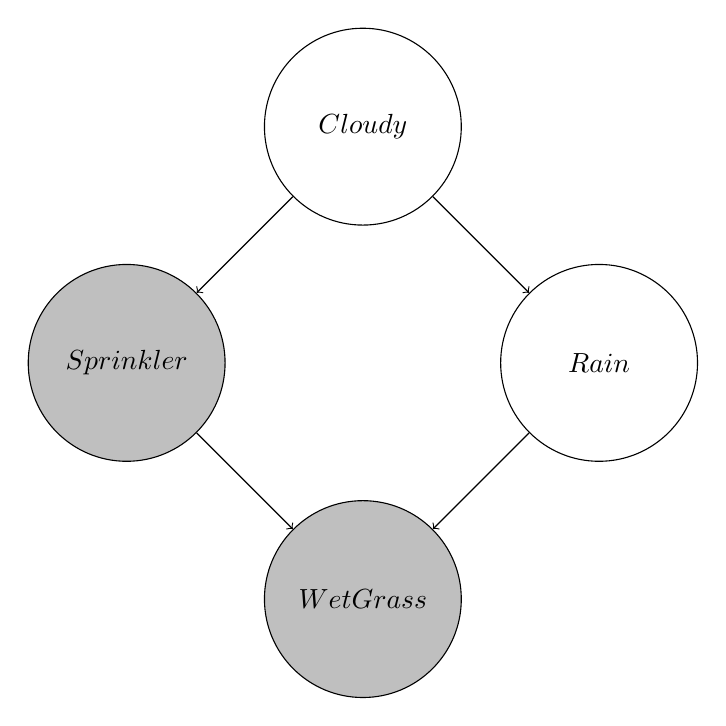
\begin{tikzpicture}
        % Nodes with fixed minimum size for equal circles
        \node (1) [circle, draw, minimum size=2.5cm] at (0, 3) {\(Cloudy\)};
        \node (2) [circle, draw, minimum size=2.5cm] at (3, 0) {\(Rain\)};
        \node (3) [circle, draw, fill=gray!50, minimum size=2.5cm] at (0, -3) {\(Wet Grass\)};
        \node (4) [circle, draw, fill=gray!50, minimum size=2.5cm] at (-3, 0) {\(Sprinkler\)};
        
        % Edges
        \draw[->] (1) -- (2);
        \draw[->] (1) -- (4);
        \draw[->] (2) -- (3);
        \draw[->] (4) -- (3);
    
    \end{tikzpicture}
\end{center}

does not satisfy the property that makes our belief propagation algorithm work. 

Therefore we need to change our strategy. One possiblity is to rely on sampling to perform approximate inference on the probability distributions we are interested in. 

The question then is how to sample from $p(x|y = \bar{y})$?

To do this we notice that we can generally compute the unnormalized probability distibution $\tilde{p}(x)$ such that 

$$
p(x) = \frac{1}{Z}\tilde{p}(x)
$$

The typical scenario where this happens is given by the Bayes Theorem 

$$
p(x|y) = \frac{p(y|x)p(x)}{p(y)}
$$

where $p(y)$ is hard to compute (can be complicated high dimensional integral).

Our sampling problem than boils down to generate samples $x_1, \dots, x_n$ from $p(x)$ knowing $\tilde{p}(x)$, as independent as possible among them. Once we have set of samples also able to estimate quantities like 

$$
\mathbb{E}[f(x)] = \int f(x)p(x)dx \approx \frac{1}{n}\sum_{i=1}^n f(x_i)
$$

We are going to see two main ways to perform this:
\begin{itemize}[label=$\blacktriangleright$, leftmargin=2em, itemindent=0em]
    \item Sample from $q(x) \approx p(x)$ and then correct. These are very common methods but they may suffer from efficiency issues. 
    \item Markov Chain Monte Carlo (MCMC), which allows us to generate a set of samples from an unnormalized distribution. 
\end{itemize}

\textbf{Remark.} Sampling is a computational intensive task and vanilla methods are not scalable to high dimensional probability distributions. 

\section{Approximate Sampling}

We are going to explore methods that allow us to sample from a surrogate $q(x)\approx p(x)$. 

\subsection*{Rejection Sampling}

Suppose to have a distribution $p(x)$ and another distribution $g(x)$ from which it is easy to sample, called the \textbf{proposal distribution}, such that $\exists M>0 : Mg(x)\geq p(x), \forall$, which of course implies that $\frac{p(x)}{Mg(x)}\leq 1$.

Rejection sampling consists in the following algorithm:
\begin{enumerate}
    \item Sample $\hat{x}$ from $g(x)$
    \item Accept $\hat{x}$ with probability $\frac{p(\hat{x})}{Mg(\hat{x})}$
    \item If reject, then repeat the algorithm until acceptance
\end{enumerate}

Graphically, once we sample $\hat{x}$, the acceptance mechanism corresponds to sample uniformly a number $\alpha$ between 0 and 1, multiply it by $Mg(x)$ and accept if and only if $\alpha Mg(x)$ falls below the original distribution at the point $\hat{x}$. We reject if the opposite happens. 

\begin{figure}[H]
    \centering
    \includegraphics[width=0.6\textwidth]{assets/fig31.png}
    \caption{In the rejection sampling method, samples are drawn from a simple distribution $g(x)$ and rejected if they fall in the grey area between the distribution $p(x)$ and the scaled distribution $Mg(x)$. The resulting samples are distributed according to $p(x)$. \cite{bishop2006pattern}}
    \label{fig:rejection_sampling}
\end{figure}

\textbf{Remark.} We can actually compute the expected number of samples from $g$ to accept a single sample on $p$, and this expectation is in fact $M$. Therefore, if $M$ is large, this method becomes inefficient. Rejection sampling is especially inefficient in high dimension (you need a large $M$ to "cover" $p$).

\textbf{Remark.} If we consider the unnormalized distribution $\tilde{p}(x)$ in place of $p(x)$ in the rejection sampling scheme, then we can use the fraction of rejected points to estimate the normalization constant $Z$. In fact,

$$
Z = \int \tilde{p}(x)\,dx = M \int \frac{\tilde{p}(x)}{Mg(x)}g(x)\,dx = M\cdot p(accept)
$$

\subsection*{Importance Sampling}
The goal in importance sampling is to evaluate

$$
\mathbb{E}_p[f(x)] = \int f(x)\frac{1}{Z}\tilde{p}(x)\,dx = \frac{\int f(x)\tilde{p}(x)\,dx}{\int \tilde{p}(x)\,dx}
$$

where $f$ if an integrable function. 

We consider a proposal distribution $g(x)$ from which we know how to sample from, and we turn the expectation on $p$ into an expectation on $g$. 

$$
\frac{\int f(x)\tilde{p}(x)\,dx}{\int \tilde{p}(x)} = \frac{\int f(x)\tilde{p}(x)\frac{g(x)}{g(x)}}{\int \tilde{p}(x)\frac{g(x)}{g(x)}} = \frac{\mathbb{E}_g\left[f\frac{\tilde{p}}{g}\right]}{\mathbb{E}_g\left[\frac{\tilde{p}}{g}\right]}
$$

Then we sample $x_1, \dots, x_n$ from $g(x)$ and replace the expectation with sums 

$$
\frac{\mathbb{E}_g\left[\frac{p}{g}\right]}{\mathbb{E}_g\left[\frac{p}{g}\right]} = \frac{\frac{1}{N}\sum_{i=1}^{N} f(x_i)w(x_i)}{\frac{1}{N}\sum_{i=1}^{N}w(x_i)}
$$

where  

$$
w(x_i):= \frac{\tilde{p}(x_i)}{g(x_i)}
$$

are known as the \textbf{importance weights}.

If $\frac{f\tilde{p}}{g}$ is approximately constant, then estimates can be very good. If weights vary a lot instead, we have a large variance and consequently a poor estimate. So, the quality of the result depends from the choice of $g(x)$. 

Notice that $\frac{1}{N}\sum_{i=1}^{N}w(x_i) \approx Z$, so we also have an approximation of the partition fraction. 

\textbf{Remark.} This technique can be used to estimate functions of rare events, increasing the probability that the event happens and then correcting it.

\begin{exampleblock}
If we want to compute $\mathbb{E}_p\left[f(x)\right]$ where $p(x) = \mathcal{N}(x;0,1)$ and $f(x) = x^{20}$, using samples from $p(x)$ would be inefficient, as the expected value is mostly influenced by extreme values of $x$. One can then use importance sampling with a Gaussian with larger variance as proposal distribution. 
\begin{figure}[H]
    \centering
    \includegraphics[width=0.8\textwidth]{assets/fig32.png}
    \caption{Importance sampling example. Sampling from $p(x) = \mathcal{N}(x;0,1)$ to compute $\mathbb{E}_p\left[f(x)\right]$ with $f(x) = x^{20}$ would be inefficient, as most of the contribution to the integral is given by values of $x$ that are rare $(|x|>3\sigma_p)$. Using as proposal distribution a Gaussian with larger variance allows us to sample from the region that contributes to the expected value.}
    \label{fig:importance_sampling}
\end{figure}
\end{exampleblock}

\section{Markov Chain}

A Markov Chain is a stochastic process, denoted as 

$$
\left\{X_t\right\}_{t\geq 0}
$$

with $t \in \mathcal{N}, X_0, X_1, \dots, X_t \in \mathcal{X}$ where $\mathcal{X}$ can be discrete or continuous. 

It can be described as a \textit{dynamical system}, i.e. a system in which we start from a certain state $x_0$ with a given probability $p_0(x)$ and that changes state according to a dynamic described by the \textit{transition kernel} $p(x_n|x_{n-1})$. 

\textbf{Remark.} Markov Chains satisfy the \textit{memoryless property}, which corresponds to the assumptions encoded into the following probabilistic graphical model:
\vspace{0.5cm}
\begin{center}
    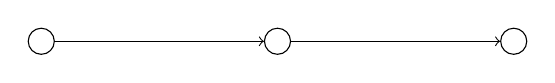
\begin{tikzpicture}
        % Nodes with fixed minimum size for equal circles
        \node (1) [circle, draw] at (0, 0) {\(\)};
        \node (2) [circle, draw] at (3, 0) {\(\)};
        \node (3) [circle, draw] at (6, 0) {\(\)};
        
        % Edges
        \draw[->] (1) -- (2);
        \draw[->] (2) -- (3);
    
    \end{tikzpicture}
\end{center}
\vspace{0.5cm}
Therefore we have that 

$$
p(x_n|x_{n-1},\dots, x_0) = p(x_n|x_{n-1})
$$

which is known as the memoryless or Markov property.

We also require the \textbf{time homogeneity} property that states that 

$$
p(x_n|x_{n-1}) = p(x_1|x_0), \forall n \geq 1
$$

which means that the probability to jump from a certain state to another state stays the same for every time step. 

\begin{definitionblock}[Transition Kernel]
    $p(x_n|x_{n-1})$ satisfying the time homogeneity property is called the (one step) \textbf{transition kernel}.
\end{definitionblock}

For a discrete state space we would have a \textit{transition matrix}, while for a continuous state space, $p(x_n|x_{n-1})$ is a probability density on $x_n$ depending continuously on $x_{n-1}$.

Since we are interested at the behaviour of the Markov Chain as the index $n$ progresses, i.e. for large times, we need to define few more concepts. 

\begin{definitionblock}[Ergodic Markov Chain]
    A \textit{Markov Chain} is \textbf{ergodic} $iff \forall x, y \in \mathcal{X}, \exists t \geq 0 : p(x_t = y|x_0 = x) > 0$.
\end{definitionblock}

If a Markov Chain is ergodic, it means that there is always the possibility of going from a given state $x$ to another given state $y$ if we are patient enough. This means that the entire state space is reachable, no matter where we start exploring. 

\begin{definitionblock}[Stationary Distribution]
    A \textbf{Stationary Distribution $\Pi(y)$} is such that
    \begin{enumerate}
        \item $$\Pi(y) = \int p(y|x)\Pi(x)\,dx$$
        
        which means that $\Pi$ is an \textbf{invariant measure} with respect to the Markov Chain dynamics defined bu the Transition Kernel $p(y|x)$
        \item $p_n(x) = p(x_n|x_0) \xrightarrow[n \to \infty]{} \Pi(x)$
        \item $\Pi$ is unique
    \end{enumerate}
\end{definitionblock}

\subsection*{Detailed Balance}

The following condition is sufficient to guarantee that $\Pi(x)$ is a stationary distribution.

\begin{definitionblock}[Reversible Markov Chain]
    We say that a Markov Chain is \textbf{reversible} (or it satisfies the \textbf{balance condition}) $iff \exists \Pi(x)$, probability distribution such that

    $$
    p(x|y)\Pi(y) = p(y|x)\Pi(x)
    $$
\end{definitionblock}

\begin{Proposition}
If an ergodic Markov Chain is reversible with respect to the distribution $\Pi(x)$, then $\Pi(x)$ is a stationary distribution.
\end{Proposition}
\begin{proof}
    If the Markov Chain is reversible then we can write 

    $$
    \int p(y|x)\Pi(x)\,dx = \int p(x|y)\Pi(y)\,dx = \Pi(y)\int p(x|y)\,dx = \Pi(y)
    $$
\end{proof}

\textbf{Remark.} It is not true that the existence of a stationary distribution implies that our Markov Chain is reversible.

We are now ready to tackle Markov Chain Monte Carlo: by requiring that the Markov Chain we are going to define satisfies the detailed balance condition for a given distribution $\Pi(x)$, we will be eventually ($t \to \infty$) able to sample from distribution of interest, i.e. $\Pi(x)$.

\section{Markov Chain Monte Carlo}

\subsection*{Metropolis Hastings}

Intuitively, the idea is that we want to sample from a distributino and we build an ergidic Markov Chain with a transition kernel such that the stationary distribution coincides with the one we want to sample from. 

Assume that we want to sample from $p(x) = \frac{1}{Z}\tilde{p}(x)$, where we know the unnormalized distirbution $\tilde{p}(x)$ but the normalization constant is too complicated to compute. We fix $q(x|y)$, the \textit{proposal kernel} of our Markov Chain, such that 
\begin{enumerate}
    \item It is easy to sample from $q(x|y)$
    \item It makes our Markov Chain ergodic
\end{enumerate}

A typical choice for our proposal kernel is to use a Gaussian distribution, in which the variance is chosen in such a way that makes it quick to reach the stationary distribution. 

Suppose that we start from a certain state $x$ at the time step $t$. 

The algorithm works as follows:
\begin{enumerate}
    \item We sample $y$ from $q(x|y)$
    \item Borrowing from rejection sampling, we are going to accept/reject the new sampled point based on the following rule 
    $$
    x_{t+1} = \begin{cases}
        y & \text{with probability } \alpha(y|x) = \min \left\{1, \frac{\tilde{p}(y)q(x|y)}{\tilde{p}(x)q(y|x)}\right\}\\
        x & \text{otherwise}
    \end{cases}
    $$
\end{enumerate}

The criterion for defining

$$
\alpha(y|x) = \min \left\{1, \frac{\tilde{p}(y)q(x|y)}{\tilde{p}(x)q(y|x)}\right\}
$$

is called the \textbf{Metropolis-Hastings} criterion; for symmetric transition kernels $q(x|y) = q(y|x)$, it becomes the Metropolis criterion.

Observe that 

$$
\frac{\tilde{p}(y)}{\tilde{p}(x)} = \frac{p(y)}{p(x)}
$$

and so the regions with higher probability $p(y)>p(x)$ are more likely to be visited.

Notice that we haven't defined in a full mathematical way the transition kernel of our Markov Chain here, but it can be derived bu the operational procedure given above. 

\newtheorem{Lemma}{Lemma}
\begin{Lemma}
The Metropolis-Hastings acceptance criterion satisfies the detailed balance condition.
\end{Lemma}
\begin{proof}
Let's start from the full transition kernel in an implicit form and suppose that $y\neq x$. Then we need to prove that 

$$
p(y|x)p(x) = p(x|y)p(y)
$$

If $y\neq x$, the first term reduces to the product of the probability to sample $y$ given $x$, which is given by $q(y|x)$, times the probability to accept $y$, which is given by $\alpha(y|x)$. Therefore 

$$
p(y|x)p(x) = q(y|x)\alpha(y|x)p(x) = \min \left\{1, \frac{\tilde{p}(y)q(x|y)}{\tilde{p}(x)q(y|x)}\right\} \cdot q(y|x)p(x)
$$

Notice that

$$
\frac{p(y)}{p(x)} = \frac{\tilde{p}(y)}{\tilde{p}(x)}
$$

Performing some calculations we obtain 

$$
\begin{array}{rl}
    \min \left\{1, \frac{\tilde{p}(y)q(x|y)}{\tilde{p}(x)q(y|x)}\right\} \cdot q(y|x)p(x) &= \min {q(y|x)p(x), p(y)q(x|y)} \\
    &= \min \left\{\frac{p(x)q(y|x)}{p(y)q(x|y)}, 1\right\} \cdot q(x|y)p(y) \\
    &= \alpha(x|y)q(x|y)p(y) \\
    &= p(x|y)p(y)
\end{array}
$$
\end{proof}

There might still be issues: if we pick a bad $q$ the algorithm may take a lot of steps before reaching the stationary distribution. We say that the \textbf{mixing time} is high. This time can be estimated by some statistics on the chain that is being sampled, that form a sort of \textit{diagnostics tools}. However, there is not a way to determine the exact moment in which the steady state is reached. Moreover, another issue is that the samples $x_n, x_{n+1}$ are not independent.

Another good property that we may want to have in our proposal kernel is to have a good balance in between exploration and exploitation, which becomes especially important in multimodal distribution.

\subsection*{Gibbs Sampling}

This time, let's write the probability distribution from which we want to sample from as $p(x) = p(x_1, \dots, x_n)$ and suppose that we know how to sample from the 1-dimensional conditionals, i.e. from $p(x_i|x_{-i})$ where $x_{-i} = (x_1, \dots, x_{i-1}, x_{i-1}, \dots, x_n)$.

The main loop of Gibbs sampling algorithm is the following:
\begin{enumerate}
    \item Pick $k\in {1, \dots, n}$
    \item Set $x_j^{(t+1)} = x_j^{(t)}$ for $j \neq k$ (the j-th component of the t+1 state)
    \item Sample $x_k^{(t+1)}$ from $\tilde{p}(x_k|x_{-k}^{(t)})$
\end{enumerate}

Therefore we are choosing a coordinate and sample along that coordinate, keeping everything else fixed. We have different ways to choose k:
\begin{enumerate}
    \item Round-Robin strategy, i.e. sample starting from 1, go up to k on the first k steps and then repeat.
    \item Choose uniformly at random.
\end{enumerate}

\begin{Lemma}
    The transition kernel of Gibbs Sampling is exactly the same as Metropolis-Hastings algorithm.
\end{Lemma}
\begin{proof}
    In fact, for Gibbs Sampling we have 

    $$
    q_k(y|x) = \begin{cases}
        p(x_k|x_{-k}) & \text{when } y_{-k} = x_{-k}\\
        0 & \text{otherwise}
    \end{cases}
    $$

    Which means that $\alpha_k(y|x) = 1$ because 

    $$
    \alpha_k(y|x) = \frac{p(y)q(x|y)}{p(x)q(y|x)} = \frac{p(y_k|y_{-k})p(y_{-k})}{p(x_k|x_{-k})p(x_{-k})}\cdot \frac{p(x_k|y_{-k})}{p(y_k|x_{-k})}
    $$

    Where the equality is given by the standard conditional probability expansion. Also notice that $x_{-k} = y_{-k}$, otherwise there would be no jump according to the definition of our proposal kernel. Then 

    $$
    \frac{p(y_k|y_{-k})p(y_{-k})}{p(x_k|x_{-k})p(x_{-k})} = \frac{p(y_k|y_{-k})}{p(x_k|x_{-k})} = 1
    $$
\end{proof}

Gibbs Sampling algorithm can be generalized, for example, by sampling blocks instead of a single variable, i.e. we can sample $x_j, \dots, x_k \subseteq x$. Moreover, we could apply this even if we don't know explicitly how to sample from $p(x_i|x_{-i})$, for example by applying rejection sampling, or even a Metropolis-Hastings MCMC to smaple our conditional distribution (the latter strategy is called "Metropolis within Gibbs").

\textbf{Remark.} 
\begin{itemize}[label=$\blacktriangleright$, leftmargin=2em, itemindent=0em]
    \item We may not satisfy ergodicity in Gibbs sampling, since it may not always be possible to find a path between two stated which is only made of "single component" steps. 
    \begin{exampleblock}
    Consider the bivariate distribution $p(x,y) = 2$ if $(x \in [0,0.5] \land y \in [0,0.5]) \lor (x \in [0.5,1] \land y \in [0.5,1]), 0$ otherwise. In this case, we cannot sample from an "island" different from the one where we start sampling.
    \begin{figure}[H]
        \centering
        \includegraphics[width=0.5\textwidth]{assets/fig33.png}
        \label{fig:gibbs_sampling_island}
    \end{figure}
    \end{exampleblock}
    \item If variables are strongly correlated, then our mixing time can be very high.
\end{itemize}

\newpage
\subsection*{Sampling based inference in PGM}

\begin{center}
    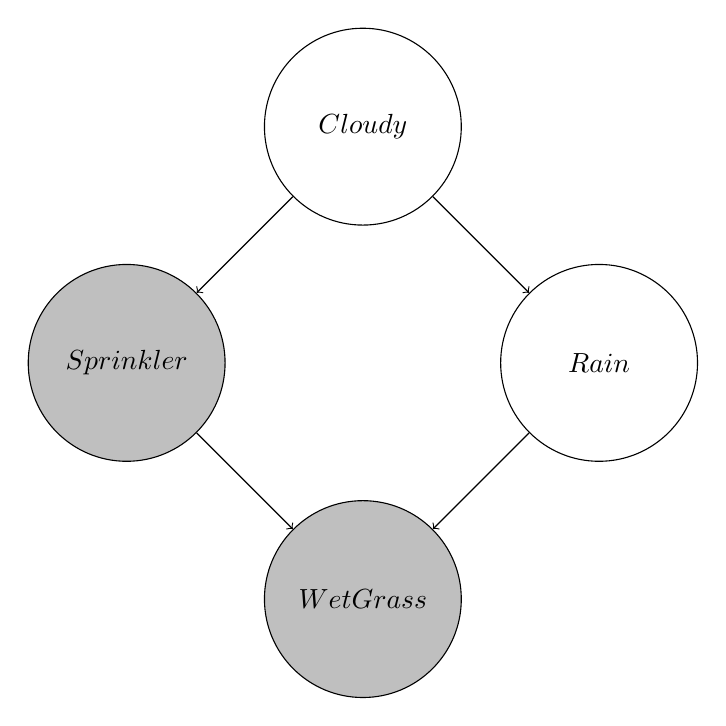
\begin{tikzpicture}
        % Nodes with fixed minimum size for equal circles
        \node (1) [circle, draw, minimum size=2.5cm] at (0, 3) {\(Cloudy\)};
        \node (2) [circle, draw, minimum size=2.5cm] at (3, 0) {\(Rain\)};
        \node (3) [circle, draw, fill=gray!50, minimum size=2.5cm] at (0, -3) {\(Wet Grass\)};
        \node (4) [circle, draw, fill=gray!50, minimum size=2.5cm] at (-3, 0) {\(Sprinkler\)};
        
        % Edges
        \draw[->] (1) -- (2);
        \draw[->] (1) -- (4);
        \draw[->] (2) -- (3);
        \draw[->] (4) -- (3);
    
    \end{tikzpicture}
\end{center}

Suppose that we observe the variables "Sprinkler" and "Wet grass", but we don't observe "Cloudy" and "Rain". 

More generally, suppose to have a set of variables (could be vector of random variables), $x$ and $y$ that are described by a PGM and we know that $y$ is observed, $y = \hat{y}$. We want to make inference on $x$, which typically means computing $p(x|y = \hat{y})$. We aim at sampling from this probability, but we do not have access to such a conditional distribution. We only know $\tilde{p}(x) = p(x, y = \hat{y})$, but not the normalization constant $X = p(y = \hat{y})$.

Here are some strategies then to generate samples from this distribution:
\begin{itemize}[label=$\blacktriangleright$, leftmargin=2em, itemindent=0em]
    \item Rejection sampling: sample from the full joint $p(x,y)$ which can be done by ancestral sampling (which is fast) and then reject if $y \neq \hat{y}$. If we observe a lot of variables then this becomes very inefficient.
    \item A better strategy is to use MCMC. We can sample from $p(x,y = \hat{y})$ using some proposal distribution (which will depend on the variables that we are trying to sample). Although the state of the art of MCMC (Hamiltonian Monte Carlo, explained later on) is generally good, in the framework of Bayesian Networks we can do better. 
    \item If we can compute efficiently the one dimensional conditional distribution, i.e. $p(x_i|x_{-i},y) = p(x_i|MB_i)$, where $MB_i$ is the Markov Blanket of $x_i$, we can use \textit{Gibbs sampling}. This is especially efficient with discrete, and relatively small state spaces. 
\end{itemize}

\subsection*{Convergence Diagnostics}

How can we check that out Markov Chain has reached the steady state? We will put forward a set of tools that can monitor one or more trajectories and roughly tell us whether we reached it or not. Notice that since we are interested in sampling the stationary probability distributions, we shall start keeping the samples only when we actually reached the steady state. 

Let's define some notation for the rest of the section. We are going to denote a general function over a state of the MCMC trajectory $(X_t)_{t\geq 0}$ as $\Psi : \mathcal{X} \to \mathbb{R}$. This function can be a lot of different things, depending on what we are interested in computing, e.g. a projection on single coordinate. 

We will assume that $\Psi$ has values in $\mathbb{R}$, and not just in a subset of it, and, if it does, we transform the function $\Psi$ to make it compliant to this assumption (taking the logarithm of quantities in between ($0, \infty$) for example). Let's fix some further notation:
\begin{itemize}[label=$\blacktriangleright$, leftmargin=2em, itemindent=0em]
    \item $x_1, \dots, x_n$ is our sampled trajectory 
    \item $\Psi_j := \Psi(x_j)$
    \item $\bar{\Psi} := \frac{1}{N}\sum_j \Psi_j$ is the estimate of $\mathbb{E}[\Psi] = \int \Psi(x)p(x)\,dx$
\end{itemize} 

On a high level, the idea is to look at more than one chain and compare the distribution of the samples that we obtain and see if they look more or less the same. 

Practically,
\begin{enumerate}
    \item We sample $\frac{m}{2}\geq 1$ trajectories from overdispersed initial points. We try to start from different states that are far away in our state space.
    \item Sample for $4n$ steps.
    \item We throw away the first half of every trajectory so that we have only $2n$ points left. This phase is known as the \textbf{burn-in} or \textbf{warm-up} phase. We do this because it takes time to reach the steady state (notice this is an heuristic: convergence to the stationary distribution can happen faster or slower than $2n$ steps).
    \item Then we split in 2 parts the remain trajectories, so that we are left with $m$ different trajectories each of length $n$.
\end{enumerate}

From now on we will denote each sample as $x_{ij}$ where $i \in [1,n]$ and $j \in [1,m]$, where this notation describes the $i_{th}$ sample of the $j_{th}$ trajectory.

We will also denote $\Psi(x_{ij}) = \Psi_{ij}$ and define 

$$
\begin{cases}
    \bar{\Psi}_j := \frac{1}{n}\sum_{i=1}^n \Psi_{ij} \\
    \bar{\Psi} := \frac{1}{m}\sum_{j=1}^m \bar{\Psi}_j
\end{cases}
$$

Hence, $\bar{\Psi}_j$ is the average within the trajectory $j$ and $\bar{\Psi}$ the average over all the trajectories, respectively. We are also interested in the variance of $\bar{\Psi}$, but since our samples are not independent, we don't have that $VAR[\bar{\Psi}] = \frac{1}{n}VAR[\Psi]$, i.e. the variance of the estimator in this case is not just the variance of our random variable divided by the number of samples. If you think about two consecutive points in the chain, there is a high chance that the correlation between them is higher than that of two points which are sampled distantly in time from one another. 

Let's define these two quantities:

$$
W := \frac{1}{m}\sum_{j=1}^m s_j^2, \quad s_j^2 := \frac{1}{n-1}\sum_{i=1}^n (\Psi_{ij} - \bar{\Psi}_j)^2
$$
$$
B := \frac{n}{m-1}\sum_{j=1}^m (\bar{\Psi}_j - \bar{\Psi})^2
$$

W is called the \textbf{within variance} while B is called the \textbf{between variance}.

We know by definition that 

$$
W \leq VAR[\Psi],
$$

because when sampling single trajectories we have not necessarily explored and visited the full space. Increasing the number of samples we will converge the true variance. Moreover, as long as the initial states are overdispersed, it can be shown that

$$
VAR[\Psi] \leq VAR^{+}[\Psi] := \frac{n-1}{m}W + \frac{1}{n}B 
$$

Then we have both a lower and an upper bound for our variance, both converging to the true variance. Therefore we can compute the statistics 

$$
\hat{R} := \sqrt{\frac{VAR^{+}[\Psi]}{W}}
$$

but unfortunately this is not the case as we have already seen.

The correlations among nearby points (when positive as typically the case) are increasing the variance of the estimator $\bar{\Psi}$, in a way which can be expressed by this formula:

$$
nmVAR[\bar{\Psi}] \approx \left(1 + 2\sum_{k=1}^{\infty}\rho_k\right) VAR[\Psi]
$$

Where $\rho_k$ is the autocorrelation of lag k, which is, by definition 

$$
\rho_k := Corr[\Psi(x_i), \Psi(x_{i+k})]
$$

So it is the correlation in between two points in the same chain which are k steps apart. 

If we compare the formula above with what we would have in case of independence, we can find the \textbf{effective number of samples} produced by our chain 

$$
n_{eff} = \frac{nm}{(1 + 2\sum_{k=1}^{\infty}\rho_k)} \leq nm 
$$

And we can also write

$$
VAR[\bar{\Psi}] = \frac{VAR[\Psi]}{n_{eff}}
$$

A typical rule of thumb here is to reach at least $n_{eff} = 100$ effective samples. 

The question now is: how do we compute the autocorrelation? We know that this identity holds (no proof given)

$$
\mathbb{E}[(\Psi_i - \Psi_{i-k}^2)] = 2(1 - \rho_k)VAR[\Psi]
$$

and since we can estimate both the left hand side term and $VAR[\Psi]$ from our data, we can also estimate $\rho_k$ by inverting the formula. 

The expectation above is named \textbf{Variogram at lag k} and can be estimated as 

$$
V_k = \frac{1}{m(n-k)}\sum_{j=1}^m \sum_{i=k+1}^n (\Psi_{i,j} - \Psi_{i-k,j})^2
$$

So that 

$$
\hat{\rho}_k = 1 - \frac{V_k}{2VAR^{+}[\Psi]}
$$

We still have problems in the limit of large k because we would have few samples and very noisy estimates. Therefore we will stop the sum over k when the following condition is satisfied

$$
T = \min{k|k \text{is odd, } \hat{\rho}_{k+1} + \hat{\rho}_{k+2} < 0}
$$

When this condition is satisfied we are in a regime where our summation is now relevant anymore. 

Therefore, we approximate the sum as 

$$
\sum_{k=1}^{\infty}\rho_k \approx \sum_{k=1}^{T}\hat{\rho}_k 
$$

In conclusion, we have two different diagnostics tool to detect convergence: either we look at an estimate of the variance and compute the factor $\hat{R}$ or we look at the number of effective samples and have an estimate of how decent our approximation is going to be.

\section{Hamiltonian Monte Carlo}

Hemiltonian Monte Carlo can be considered as the state of the art method for doing Markov Chain Monte Carlo. It falls into the category of \textit{augmented varibles} Monte Carlo methods.

The idea it to turn the problem into an Hemiltonian, augmenting the state space with momentum variavbles that provide a sort of "kinetic energy" that allows the algorithm to move along the surface of the energy corresponding to our probability distribution. This scheme improves a lot of the mixing time, hence the efficiency of MCMC algorithms. Moreover, it can be used in the case of high-dimensional multimodal distributions because it does not remain stuck in a single mode. 

As usual, we start in a situation in which we want to sample from $p(x) = \frac{1}{Z}\tilde{p}(x)$, and now we express our distribution as 

$$
\frac{1}{Z}\tilde{p}(x) = \frac{1}{Z_x}\exp(H_x(x))
$$

This procedure is called the \textit{Boltzmann Trick} and it is always possible (just take the logarithm of the distribution) and turns our probability distribution in the form of an energy. 

Then, we introduce momentum variables $y$, as many as the number of $x$ variables that we have, and we assign them the probability distribution $p(y) = \frac{1}{Z_y}\exp(H_y(y))$, where is typical to make the assumption

$$
H_y(y) = \frac{1}{2}y^ty 
$$

i.e. to consider $p(y)$ a standard Gaussian. 

We are going to sample from the joint distribution, exploiting the independence of our variables

$$
p(x,y) = p(x)p(y) = \frac{1}{Z_xZ_y}\exp(H_x(x) + H_y(y)) = \frac{1}{Z}\exp(H(x,y))
$$

The idea of the algorithm is to sample from $p(x,y)$ and then forget about $y$. But how do we sample? We are going to sample according to the force field defined by the Hamiltonian, i.e. along lines which keep the energy constant. This means that, given some velocity, we follow a trakectory on the probability distribution space accordingly to the equation of motion in order to explore the space without losing energy. In fact, we would like to preserve energy because we want to move between regions with high probability. 

Hence we have the following algorithm:
\begin{enumerate}
    \item We start from point $x_i$
    \item We sample $y \sim p(y)$, i.e. we randomize the momentum 
    \item We choose a random direction in time, i.e. sample from \{-1,1\} 
    \item We move according to Hamiltonian dynamics from $(x_i,y)$ to a candidate $(x',y')$ doing L steps 
    \item We introduce the following rejection criterion: we accept if $H(x',y') > H(x,y)$, otherwise we accept with probability $\exp(H(x',y')) - H(x,y)$
\end{enumerate}

Moving accordingly to Hamiltonian dynamics means to move from $(x,y)$ to $(x',y')$ keeping $H(x',y') = H(x,y)$. At each step we set $(x',y') = (x + \Delta x, y + \Delta y)$ and Taylor expand the Hamiltonian 

$$
H(x + \Delta x, y + \Delta y) \approx H(x,y) + \nabla_x H_x(x)^T \Delta x + \nabla_y H_y(y)^T \Delta y 
$$

Then, enforcing the condition $H(x',y') = H(x,y)$, we can derive the equations for our movement:

$$
\begin{array}{c}
    \Delta x = \epsilon \nabla_y H_y(y) \\
    \Delta y = -\epsilon \nabla_x H_x(x)
\end{array}
$$

and we do L steps of this dynamics to find $(x',y')$.

Notice that, even if in principle we require the Hamiltonian to stay constant (and in that case we would always accept because $\exp(H(x',y') - H(x,y)) = \exp(0) = 1$), there are still numerical integration errors introduced by the approximation above which actually let us change the value of the Hamiltonian, hence we need to define the acceptance criterion as above to ensure that the dynamics compensate this error. 

\textbf{Remark} Since we are required to compute gradients, Hamiltonian Monte Carlo works only for continuous variables. The advantage of exploiting gradient information is similar to the one in gradient based optimizers (gradient descent).

\textbf{Remark} Our acceptance criterion is, in fact, Metropolis acceptance criterion 

$$
\alpha = \min \left\{1, \frac{p(x',y')}{p(x,y)}\right\} = \min {1, \exp(H(x',y') - H(x,y))}
$$

Additional heuristics, like the \textit{no-u-turn} Hamiltonian Monte Carlo, are the state of the art of Monte Carlo methods.

\textbf{Remark} The number of effective samples is higher than standard MCMC, because with Hamiltonian Monte Carlo we take larger steps.

\begin{figure}[H]
    \centering
    \includegraphics[width=0.8\textwidth]{assets/fig34.png}
    \label{fig:hamiltonian_monte_carlo}
\end{figure}


